\documentclass[a4paper]{article}

\usepackage{amssymb}
\usepackage{graphicx}
\usepackage{apacite}
\usepackage{amsmath}
\usepackage{indentfirst}
\usepackage{subcaption}
\usepackage{listings}
\usepackage [utf8] {inputenc}
\setkeys{Gin}{width=\linewidth}
\pagestyle {plain} \textwidth=145mm \textheight=255mm
\oddsidemargin=5mm \evensidemargin=5mm \voffset=-15mm

\setcounter {page}{1}

\begin{document}

\begin {center}{\bf\Large  Adaptation of the WORLD framework for frame-by-frame real-time speech analysis} \end {center}

\begin{center}
{\bf Eugene V. Koshel}

Department of Applied Mathematics

Dnipro National University, Gagarin's avenue, 72 

49010, Dnipro, Ukraine 

{\tt eugenefade@gmail.com}
\end{center}

\noindent{\bf Abstract}. WORLD is a vocoder-based speech synthesis system developed by M. Morise et al. and implemented in C++. It was demonstrated to have improved performance and accuracy when compared to other algorithms. However, it turned out to not perform well in certain scenarios, particularly, when applying the framework to very short waveforms on a frame-by-frame basis. This paper reviews the issues of the C++ implementation of WORLD and proposes modified versions of its constituting algorithms that attempt to mitigate those issues. The resulting framework is tested on both synthetic signals and on real recorded speech.

\vspace{3mm}
\noindent {\bf Key words:} speech analysis, speech synthesis, real-time signal processing, spectral envelope, $F_0$ estimation

\section{Introduction}

The speech analysis and synthesis were always popular subjects of interest for many researchers. The techniques and methods of working with speech signals developed over the last decades are now used in a variety of applications such as text-to-speech (TTS) synthesis, speaker identification (SI), voice conversion (VC), speech to text (STT) recognition, and others. One important characteristic of these applications share is that they have to operate with real-time constraints. A TTS system has to produce output from the user-provided text with minimum lag, a SI has to identify speakers quickly, a VC system should be able to operate on a signal and produce continuous output with minimal latency, etc.

There are systems of each type that satisfy these requirements and produce acceptable results. One of such systems is the WORLD framework for high-quality speech analysis and synthesis \cite{WORLD}. WORLD is a vocoder-based speech synthesis system that decomposes the speech signal into a fundamental frequency ($F_0$) using the DIO algorithm \cite{DIO}, a spectral envelope using the CheapTrick method \cite{CheapTrick}, and an excitation signal using PLATINUM algorithm \cite{PLATINUM}. Each of these components is usually estimated for every millisecond of the speech signal, forming a contour of estimations. The original signal can then be resynthesized by convolving the minimum phase response of the spectral envelope with the excitation signal. The diagram of WORLD framework is illustrated in Figure \ref{fig:WORLD_diagram}. Speech resynthesized in this way was shown to be of high quality in terms of waveform similarity with the input signal.

Unlike systems that perform direct sequence-to-sequence conversion on raw audio and usually utilize neural networks and deep learning for modeling non-linear mappings for speech-to-speech \cite{VC1, VC2}, text-to-speech \cite{WaveNet, DeepVoice3}, or speech-to-text \cite{STT1, STT2} conversions, frameworks like WORLD rely on conventional tools, are highly customizable, and make for a great basis for developing new systems.

\begin{figure}
    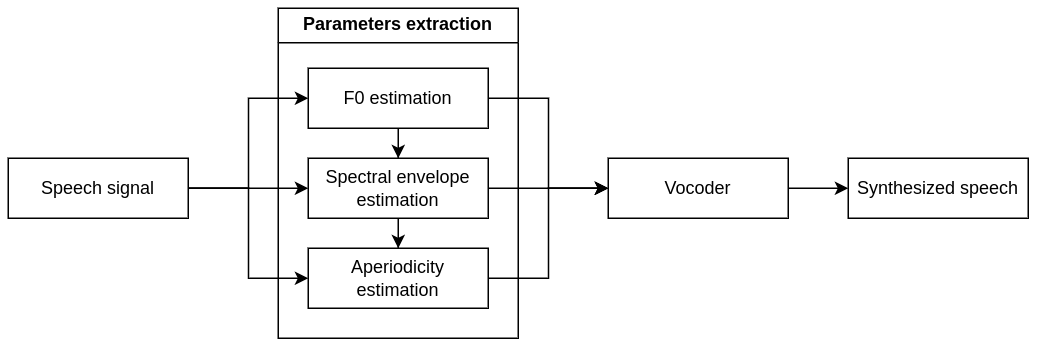
\includegraphics{graphics/WORLD_diagram.png}
    \caption{WORLD framework diagram. The original signal is decomposed into three components that are used to drive the vocoder and produce high-quality speech.}
    \label{fig:WORLD_diagram}
\end{figure}

Unfortunately, the C++ implementation of WORLD is ill-suited for one specific but very popular use case -- frame-by-frame real-time processing of audio signals. This type of processing is common in digital audio systems and used ubiquitously in music production, recording, and sound design. Such systems include, for example, Jack audio server for Linux -- a system that is intended for environments in which low latency (up to 5ms) is critical \cite{JACK}. Jack operates by connecting audio sources to audio sinks and passing pieces of signal between them using very small buffers that usually contain from 64 to 1024 samples depending on the configuration. WORLD requires buffers that are at least three times longer than the period of the lowest signal the system is expected to correctly process. So, if the speech signal is expected to have the lowest pitch of 60Hz or have period of 16ms, then the input should be at least 50ms long or contain at least 800 samples at the 16 kHz sampling rate. Jack usually doesn't provide such long buffers, but this can be solved by allocating a buffer of required size and outputting only silence while it is filling up. This approach will not impact the overall latency but will introduce delay between the first non-silent input and the first non-silent output. Even with this approach however, the WORLD framework fails at the very first stage -- the $F_0$ estimation. It either crashes or provides incorrect estimations after which all the other stages of sound decomposition are impossible. If the buffer sizes are increased significantly (above about 2000 samples), the algorithm succeeds at estimating the $F_0$ but the following stage, the spectral envelope estimation, produces unstable and noisy results that introduce heavy distortion when the sound is resynthesized.

The following sections propose alternative algorithms to those implemented in WORLD in order to enable the framework to work in the environment described earlier.

\section{$F_0$ estimation}

Fundamental frequency or pitch estimation is a process that determines the minimum frequency at which the analyzed waveform repeats itself. There are multiple and very different approaches to estimating $F_0$ of a given signal. These approaches can be broadly categorized into spectrum- and time domain-based methods. The spectrum-based methods focus on detecting peaks and distances between them in the spectral envelope or the cepstrum of the signal while the time domain-based methods attempt to detect periods between peaks and zero crossings of the raw signal in the time domain \cite{PitchDetection}. When selecting a $F_0$ detection method for a particular application multiple factors must be taken into account, such as the algorithm's accuracy to performance ratio, the expected noise level of the signal, the time constraints, required signal frame length, etc. It was shown that spectrum-based algorithms perform better than the time domain-based ones \cite{PitchDetectionPerformance}, but their drawback is that they introduce extra computation cost by requiring the spectrum or cepstrum to be computed for each frame of the signal. For this reason, the WORLD framework uses the time domain-based DIO algorithm for estimating $F_0$ quickly and cheaply. However, the C++ implementation of DIO prevents WORLD from supporting the frame-by-frame analysis and synthesis. This section discusses the adaptation of DIO to enable this support.

As the basis of the reimplementation, the improved version of DIO was selected \cite{YamahaDIO} and modified to make it work with short speech frames. The implementation itself was done in Julia programming language to make it easier to apply in data exploration scenarios. Below the detailed description of the final algorithm is provided. Our implementation of DIO will be referred to as JDIO, the algorithm by Daido and Hisaminato will be referred to as YDIO, and the C++ implementation from the WORLD framework will be referred to as CDIO in the text below.

DIO's basic idea is to narrow down the possible pitch values as much as possible, detect the most stable $F_0$ candidates for a given frame, and then select one candidate that preserves the smoothness of the corresponding voiced region's $F_0$ contour the best. The first step can be thought of as preprocessing, and it includes decimating (downsampling) the input signal so that its sample rate is just enough to represent the highest desirable frequency accurately, removing the DC component from the decimated signal, and applying parallel cascading lowpass filters to attenuate harmonics and make the low pitch detection more reliable. So, the preprocessing produces a collection of signals that have a significantly reduced number of samples due to decimation, have mean amplitude of zero, and differ only by the increasingly aggressive lowpass frequency cutoff. The second step involves applying a period detector to each of these signals and assessing the stability of a period detected in each of them. The final step simply selects one of the detected candidates based on a number of heuristics that minimize the deviation from the $F_0$ estimate for the previous frame. The flowchart representation of the algorithm is given on Figure \ref{fig:DIO_diagram}.

\begin{figure}
    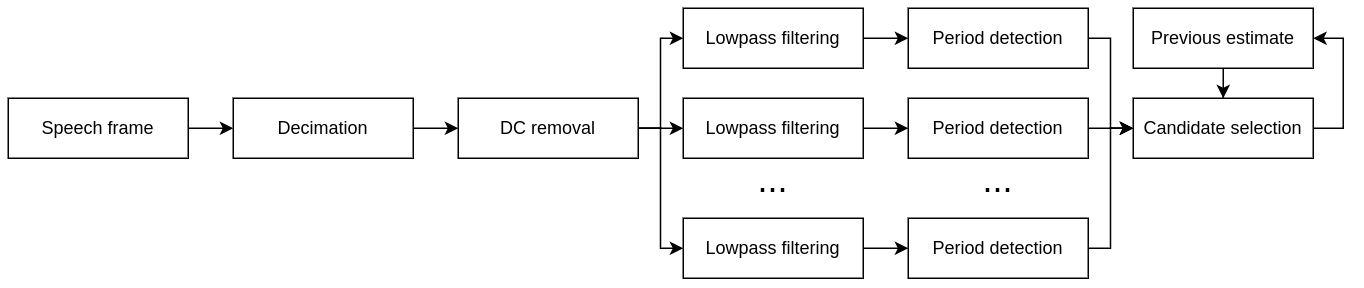
\includegraphics{graphics/DIO_diagram.png}
    \caption{Top-level representation of the DIO algorithm. Each component can be tweaked to achieve optimal performance for a given application.}
    \label{fig:DIO_diagram}
\end{figure}

In JDIO, the decimation, DC component removal, and the lowpass filtering steps were delegated to the DSP.jl package routines \cite{DSP}, while the period detection and candidate selection were implemented using custom algorithms.

Just like in YDIO, the JDIO's period detection is based on marching through the signal and identifying time durations between pairs of events of 4 types: positive zero crossings, positive peaks, negative zero crossings, and negative peaks. To make identification of these events more reliable, each of them is searched for one after the other in the provided order and in circular fashion, i.e. after detecting the negative peak, the algorithm starts searching for positive crossing. Once an event is detected at time $t_j$, the new search starts at $t_j + \tau_{\min}$. If the new search fails to find any new events until $t_j + \tau_{\max}$, the search is considered failed. $\tau_{\min}$ and $\tau_{\max}$ are constants that put hard lower and upper bounds on the range of frequencies the algorithm can detect. The search process stops once 8 successful detections have been performed, i.e. when two points of each event type have been found, and a sequence of detected timestamps $ \left[ t_1, t_2, \dots, t_8 \right] $ is obtained. From these timestamps, event periods for each event type can be calculated: $p_i = t_{i+4} - t_i, \forall i \in [1..4]$. The process of the period detection is visualized on the Figure \ref{fig:period_detection}. The estimated fundamental period of the frame is then given by the average of the periods of each event type:

\begin{equation}\label{estimated_f0}
    P_0 = \frac{1}{4} \sum_{i=1}^{4} p_{i} \quad \Rightarrow \quad F_0 = \frac{1}{P_0}.
\end{equation}

Each estimation \eqref{estimated_f0} is assigned a ``confidence'' value given by how much each event period deviates from their average value:

\begin{equation}\label{estimate_confidence}
    \lambda = 1 - \min \left[ 1, \frac{\sum_{i=1}^{4} |p_i - P_0|}{4P_0} \right].
\end{equation}

The estimates with confidence lower than a given threshold $\lambda_{\min}$ are rejected, the best $F_0$ candidate is selected among the remaining estimates.

Even though the base algorithm is fairly straightforward, its real world application presents a number of additional challenges.

First, the peak detection can suffer from a high number of false positives when the signal is noisy or contains harmonics. To mitigate this problem to some extent, two thresholds are introduced -- noise floor $0 < \eta < 1$ and relative peak amplitude $0 < \alpha < 1$. A peak point candidate $s_j$ is skipped during the peak detection process if its amplitude is lower than the noise floor or does not reach at least $\alpha$ fraction of the previous peak of the opposite sign:

\begin{equation}\label{eqn:peak_criterion}
    |s_j| > \eta \quad \land \quad |s_j| > |\alpha s_{\text{prev. peak}}|.
\end{equation}
The noise threshold also automatically filters out any unvoiced regions that otherwise would have to be identified and removed by other means.

Second, the signal being processed is discrete and the points in time at which it's sampled generally speaking do not align with the true peaks and zero crossings. This issue becomes even worse when the signal is decimated and its sampling rate is reduced significantly. An example of this is provided on the Figure \ref{fig:peak_detection}. To somewhat mitigate this issue, linear and quadratic interpolations can be used. Since zero crossings are detected by searching two consecutive points $(t_j, s_j)$ and $(t_{j+1}, s_{j+1})$ on the opposite sides of the X axis, the true zero crossing can be estimated by linearly interpolating between them and solving for zero:

\begin{equation}\label{eqn:zero_crossing}
    t_\text{zero} = -s_j\frac{t_{j+1} - t_j}{s_{j+1} - s_j} + t_j.
\end{equation}
For detecting peaks, three consecutive points $(t_{j-1}, s_{j-1})$, $(t_j, s_j)$, and $(t_{j+1}, s_{j+1})$ that satisfy the condition $ s_{j-1} < s_j > s_{j+1} $ have to be found. The true peak has to be greater than or equal to the middle point $(t_j, s_j)$ and to approximate it, a quadratic interpolation can be used. In other words, a parabola can be fitted to the three points and its extremum selected as a true peak estimate:

\begin{equation}\label{eqn:quad_interp}
    \begin{array}{l}
        \begin{bmatrix}
            t_{j-1}^2 && t_{j-1} && 1 \\
            t_j^2 && t_j && 1 \\
            t_{j+1}^2 && t_{j+1} && 1
        \end{bmatrix}
        x
        = \begin{bmatrix}
            s_{j-1} \\ s_j \\ s_{j+1}
        \end{bmatrix} \\
    \end{array}
\end{equation}
The $a$, $b$, and $c$ coefficients for $f(x)=ax^2+bx+c$ equation are given by the solution of the equation \eqref{eqn:quad_interp}. They can be used to obtain the coordinates of the fitted curve's extremum:
\begin{equation}\label{eqn:peak_detection}
    \begin{array}{l}
        t_\text{peak} = -b / 2a \\
        s_\text{peak} = -b^2 / 4a + c
    \end{array}
\end{equation}
It is important to also calculate the amplitude value $s_\text{peak}$ to use it in the condition \eqref{eqn:peak_criterion} check during the next peak detection.

Third, since there are multiple period detectors being applied in parallel to the same signal filtered with different lowpass filters as pictured in Figure \ref{fig:DIO_diagram}, multiple $F_0$ candidates $C=\left\{c_1,c_2,\dots,c_k\right\}$ are obtained, and the candidate selection procedure has to be put in place. JDIO uses the approach that minimizes the difference between the previous estimate and the new one:
\begin{equation}\label{eqn:new_f0_selection}
    F_{n+1} = c : \min_{c \in C}{\left|c - F_n\right|}.
\end{equation}
The confidence of the new estimates is guaranteed to be acceptable because all candidates with confidence lower than $\lambda_\text{min}$ are rejected. This approach helps to prevent frequency halving and frequency doubling errors for harmonic signals.

\begin{figure}
    \begin{subfigure}[b]{0.5\textwidth}
        \centering
        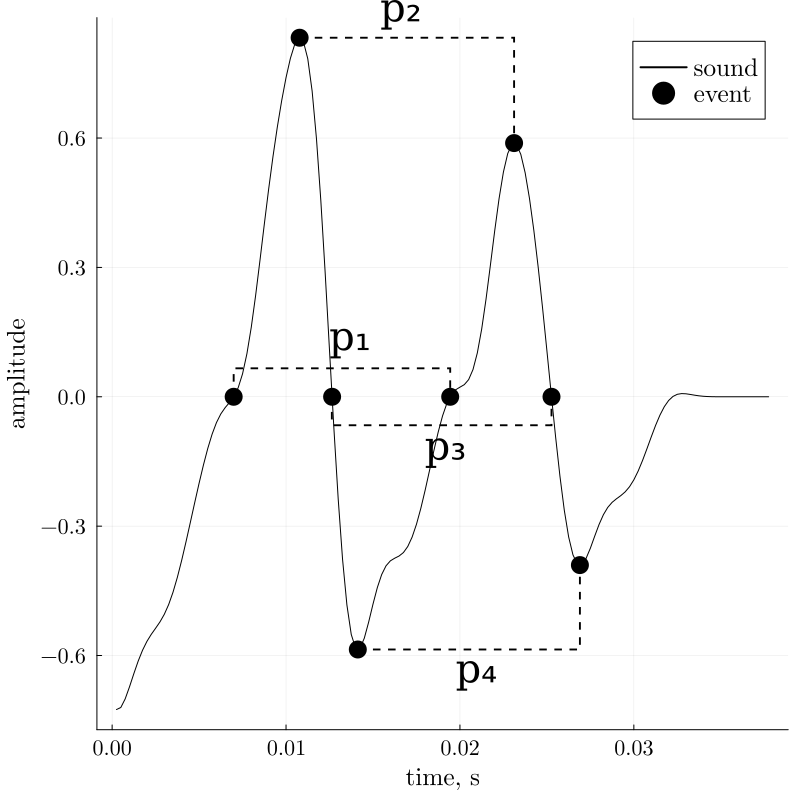
\includegraphics{graphics/pd1.png}
        \caption{}
        \label{fig:period_detection_1}
    \end{subfigure}
    \begin{subfigure}[b]{0.5\textwidth}
        \centering
        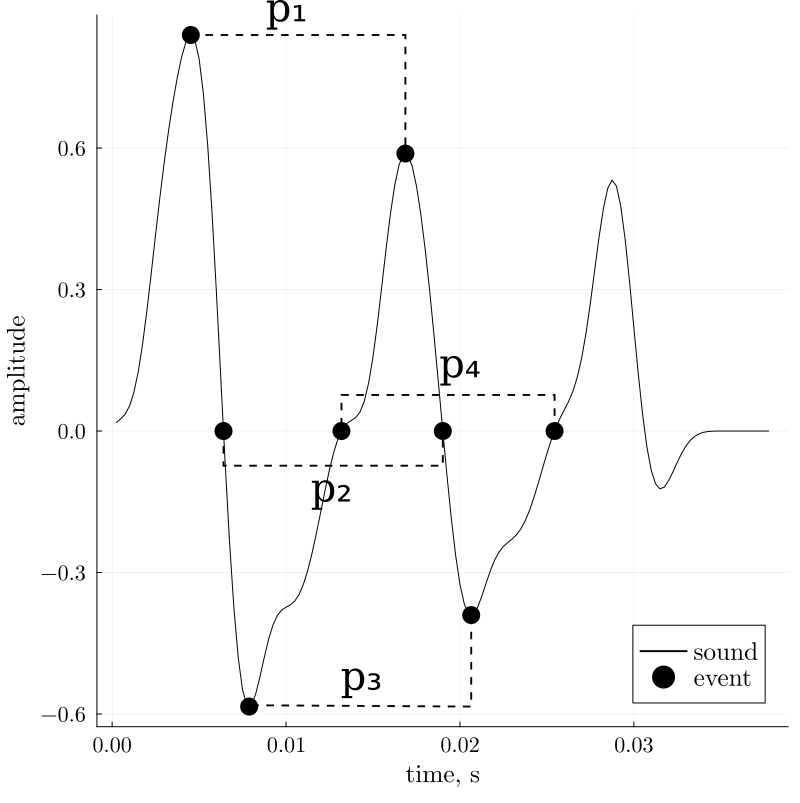
\includegraphics{graphics/pd2.png}
        \caption{}
        \label{fig:period_detection_2}
    \end{subfigure}
    \caption{JDIO detects periods between different kinds of events from a frame of signal.}
    \label{fig:period_detection}
\end{figure}

Four, since the DIO algorithm is usually used for estimating frequency contours for frames with a very short hop time, it is necessary to ensure that the event detection chain starts as close to the start of the frame as possible. To achieve this, JDIO runs each event detector and selects the one that succeeds earlier than all others. The example of different detectors being selected as first ones in the chain can be seen on the Figure \ref{fig:period_detection}. In \ref{fig:period_detection_1}, the first detected event is a positive zero crossing while in \ref{fig:period_detection_2}, the first detected event is a positive peak that satisfies the condition \eqref{eqn:peak_criterion}. In both cases, the algorithm was able to detect the best chain of events that is closest to the start of the frame and estimate the $F_0$ successfully.

\begin{figure}
    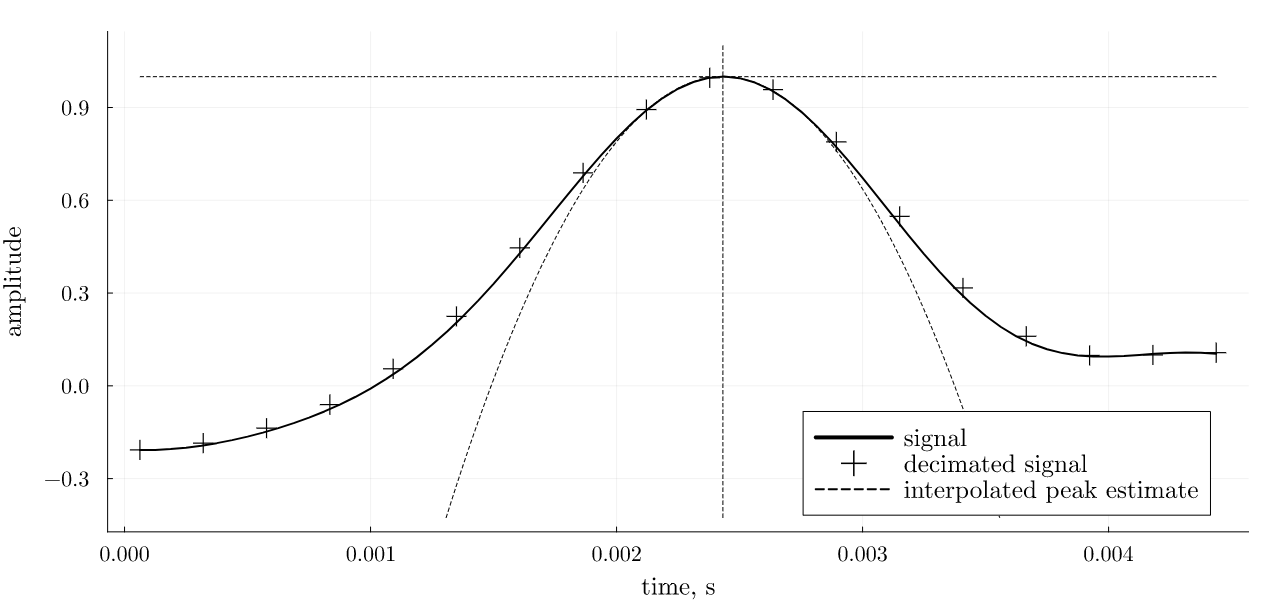
\includegraphics{graphics/peak_detection.png}
    \caption{Positive peak detection. A parabola is fitted to three points that are known to be around the true peak, and the first coordinate of its extremum is selected as the time value at which the true peak occurs.}
    \label{fig:peak_detection}
\end{figure}

\section{Spectral envelope estimation}

A spectral envelope is a curve in the frequency-amplitude plane, derived from a Fourier magnitude spectrum. The spectral envelope should ideally be a smooth line with minimal oscillations that wraps tightly around the magnitude spectrum, linking the peaks \cite{SpectralEnvelope}. In most signal processing applications, the spectrum is derived from a short frame of the signal that was windowed and padded for optimal frequency resolution in a procedure known as a short-time Fourier transform (STFT). The power spectrum estimations performed on consecutive overlapping equally sized frames of the signal comprise a spectrogram. A spectrogram represents the change of sound quality over time but because of its high frequency resolution it may contain redundant information and noise. Estimating a spectral envelope for each STFT helps to smooth the spectrum and present a clearer picture of how the large structures in the signal change over time. Spectral envelope is also easier to represent parametrically which can be used for efficient signal compression and reliable feature extraction \cite{ParametricsApplication}.

WORLD uses the CheapTrick algorithm for estimating the spectral envelope for each frame of the signal. A version of the algorithm is a part of the WORLD's C++ implementation and will be referred to as CCheapTrick in the below text. CCheapTrick works well for pre-recorded sound files, but it is not suited for real-time application because for short audio frames, it produces misaligned or noisy output that results in distortion in the reconstructed signal. Comparison of CCheapTrick's performance on real-time signal and pre-recorded audio file is shown on Figure \ref{fig:ccheaptrick}.

\begin{figure}
    \begin{subfigure}[b]{0.5\textwidth}
        \centering
        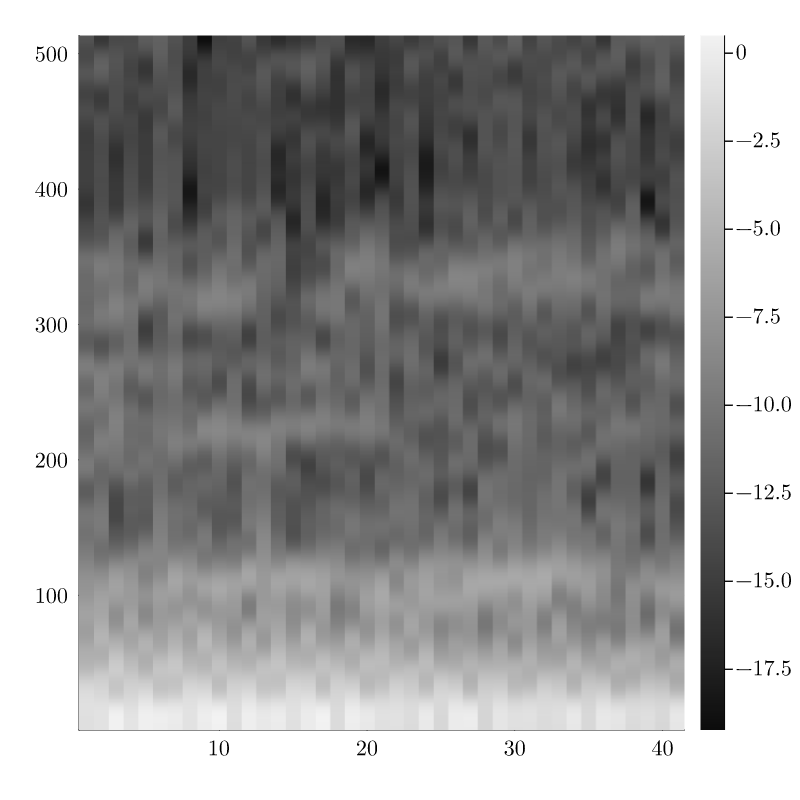
\includegraphics{graphics/realtime_ccheaptrick.png}
        \caption{}
        \label{fig:realtime_ccheaptrick}
    \end{subfigure}
    \begin{subfigure}[b]{0.5\textwidth}
        \centering
        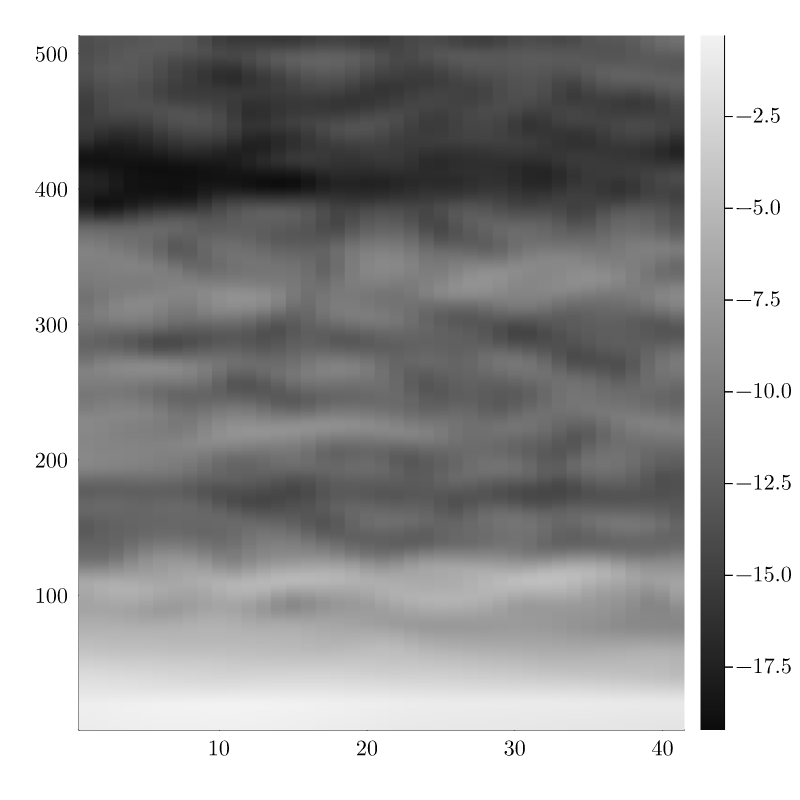
\includegraphics{graphics/recorded_ccheaptrick.png}
        \caption{}
        \label{fig:recorded_ccheaptrick}
    \end{subfigure}
    \caption{CCheapTrick is used to estimate the spectral envelope for each frame of real-time audio stream (a) and for pre-recorded audio file (b) of the same speech fragment.}
    \label{fig:ccheaptrick}
\end{figure}

A new solution, JCheapTrick, was implemented using the Julia programming language to enable analysis of real-time signals when used in conjunction with JDIO for $F_0$ estimation. Below is the detailed description of the algorithm and motivation behind the choices made during investigation and implementation.

The CheapTrick algorithm is based on adaptive signal windowing that adjusts the window size based on the instantaneous frequency of the current frame. The window itself is a regular Hann window which is given by a squared cosine in range $[-0.5,0.5]$. The window size is selected to be three times the period of the fundamental frequency $w_n = 3f_s F_0^{-1}$. For example, if a frame that is being analyzed has length of 800 samples at 16 kHz sampling rate and its instantaneous frequency is 220 Hz, the window size will be 218 which means only 218 first samples from the frame will be used for calculating its spectrum. This approach helps to ensure that the fundamental frequency and its harmonics will be the main contributors to the resulting spectrum since the instantaneous frequency is detected as close to the frame's beginning as possible as illustrated in Figure \ref{fig:period_detection}. The truncated frame with the Hann window applied to it is then padded with zeros to make its Fourier transform have sufficient resolution. The resolution is selected once and used for all frames and all window sizes to make it possible to combine all spectra into a spectrogram with consistent dimensions.

After the spectrum of a frame has been calculated, its magnitude is adjusted by the sum of the Hann window to accurately represent the energy of the frame. The adjusted spectrum then goes through a series of smoothing transformations.

First transformation is a simple FIR filter with a rectangular window. The length of the window is selected to be the index of the spectrum's energy bin which the estimated $F_0$ falls into. So, a spectrum with lower associated instantaneous frequency will be smoothed with a smaller window than the one with a higher $F_0$. In other words, the smoothing window size is selected so that it is not greater than the distance between the fundamental frequency's harmonics. The window is applied twice in forward and reverse directions to ensure that the result has zero phase distortions, i.e. the original spectrum does not shift in either direction after filtering. The added benefit of this step is that it helps to eliminate zero values from the spectrum which ensures that the cepstrum can be calculated without running into singularity issues.

The second transformation is application of the composite liftering function to the cepstrum of the signal to obtain the resulting spectral envelope.

The cepstrum is a ``power spectrum of the power spectrum'' that is calculated by applying a Fourier transform to the logarithm of the power spectrum as if it was a regular signal. Just like the spectrum helps to visualize and identify periodicities in time domain signals, cepstrum identifies periodicities in the spectrum itself. For example, a harmonic signal with a fundamental frequency of $F_0$ = 220 Hz will have a power spectrum with evenly spaced peaks that indicate $F_0$ and its harmonics; a cepstrum calculated for this power spectrum will have a peak at $F_0^{-1}$ indicating the strong periodicity in the power spectrum. The $F_0^{-1}$ value is referred to as quefrency, and it reflects a period of the corresponding frequency in the spectrum. Since the cepstrum is a regular Fourier transform, all techniques that can be applied to spectrum are also valid for cepstrum. For example, it is possible to apply a lowpass or highpass filters to the cepstrum to change the characteristics of the spectrum it was calculated for. Filters applied to the cepstrum are referred to as lifters and the process of applying them is called liftering.

The CheapTrick algorithm uses the following liftering functions:

\begin{equation}\label{eqn:smoother}
    l_s(\tau) =  \begin{cases}
        \dfrac{\sin(F_0 \pi \tau)}{F_0 \pi \tau} & \text{if $\tau > 0$} \\
        1 & \text{if $\tau = 0$}
    \end{cases},
\end{equation}
\begin{equation}\label{eqn:recoverer}
    l_q(\tau) = q_0 + 2q_1\cos(2 \pi \tau F_0).
\end{equation}
Here $\tau$ is the quefrency value, $q_0$ and $q_1$ are constants that were optimized to have values $1.18$ and $-0.9$ respectively. The function \eqref{eqn:smoother} is effectively a lowpass filter for the spectrum that removes all components that correspond to $F_0$ and its harmonics, but it also removes the temporal instability in the spectrum caused by windowing the waveform and convolutions. The function \eqref{eqn:recoverer} makes sure that the requirements of the consistent sampling theory are met, namely, that the digital signal must not change after being converted to analog signal and back. Since both of these functions are computationally expensive, the JCheapTrick implementation only computes their values up to the $F_0^{-1}$ quefrency and sets all higher values to zero. So the final liftering function is given by the equation:
\begin{equation}\label{eqn:lifter}
    L(\tau) = \begin{cases}
        l_s(\tau)l_q(\tau) & \text{if $\tau < F_0^{-1}$} \\
        0 & \text{if $\tau \geq F_0^{-1}$}
    \end{cases}.
\end{equation}
Application of this lifter yields a temporally stable spectral envelope.

\section{Evaluation}

JDIO's and JCheapTrick's implementation is meant to provide an alternative to CDIO and CCheapTrick to enable real-time applications without compromising quality and accuracy, but the fact that CDIO and CCheapTrick are unable to work with short audio frames makes the direct comparison impossible. Instead, the test audio files are processed as is by the C++ versions of the algorithms that produce an $F_0$ contour and a spectrogram respectively while the Julia algorithms operate on the same files frame-by-frame as if they were real-time streams and the outputs are concatenated to enable side-by-side comparison of $F_0$ contours and spectrograms.

For comparing the quality and accuracy of $F_0$ estimation, a number of synthesized signals was generated. Below is the table that lists total mean square errors of CDIO and JDIO on different kinds of signals with length of 1 second and the sampling rate 16 kHz.

\begin{table}[h]
    
    \begin{tabular*}{\textwidth}{@{\extracolsep{\fill}}lccl@{}}
        \hline
        Signal & JDIO & CDIO \\
        \hline
        Constant pitch signal & 0.003 & 242.0 \\
        Amplitude modulated constant pitch signal & 0.008 & 242.0 \\
        Linear chirp signal from 60 Hz to 600 Hz & 7.8 & 20.4 \\
        Amplitude modulated linear chirp & 7.8 & 20.5 \\
        Amplitude modulated linear chirp with harmonics & 67.3 & 20.7 \\
        Noisy modulated linear chirp with harmonics & 14716.1 & 25517.0 \\
        \hline
    \end{tabular*}

    \caption{Mean square deviations of the JDIO and CDIO estimations from the true $F_0$ of constant and modulated signals.}
\end{table}

From the provided numbers it seems like the accuracy of CDIO is increasing as the signals become more complex until noise is introduced and the opposite is happening with JDIO. However, the actual distribution of errors throughout the signal shows that the CDIO's accuracy is consistent in all tests and the main contributors to high error values are the estimates at the beginning and at the end of the $F_0$ contour. Such errors can be explained by the multistage postprocessing that CDIO uses to select valid $F_0$ from all the candidates it estimated for each frame of the signal -- candidates at the start and at the end of the signal lack the context for the postprocessing to work properly. Values of $F_0$ that the CDIO estimated in the middle of the signal are highly accurate, but this accuracy slowly decreases towards higher frequencies. JDIO, on the other hand, doesn't employ any form of postprocessing aside from the consecutive $F_0$ difference minimization step described in \eqref{eqn:new_f0_selection} and has better consistency in its estimates. The graphical representation of error distributions is provided on Figure \ref{fig:f0_estimations}.

\begin{figure}
    \begin{subfigure}[b]{\textwidth}
        \centering
        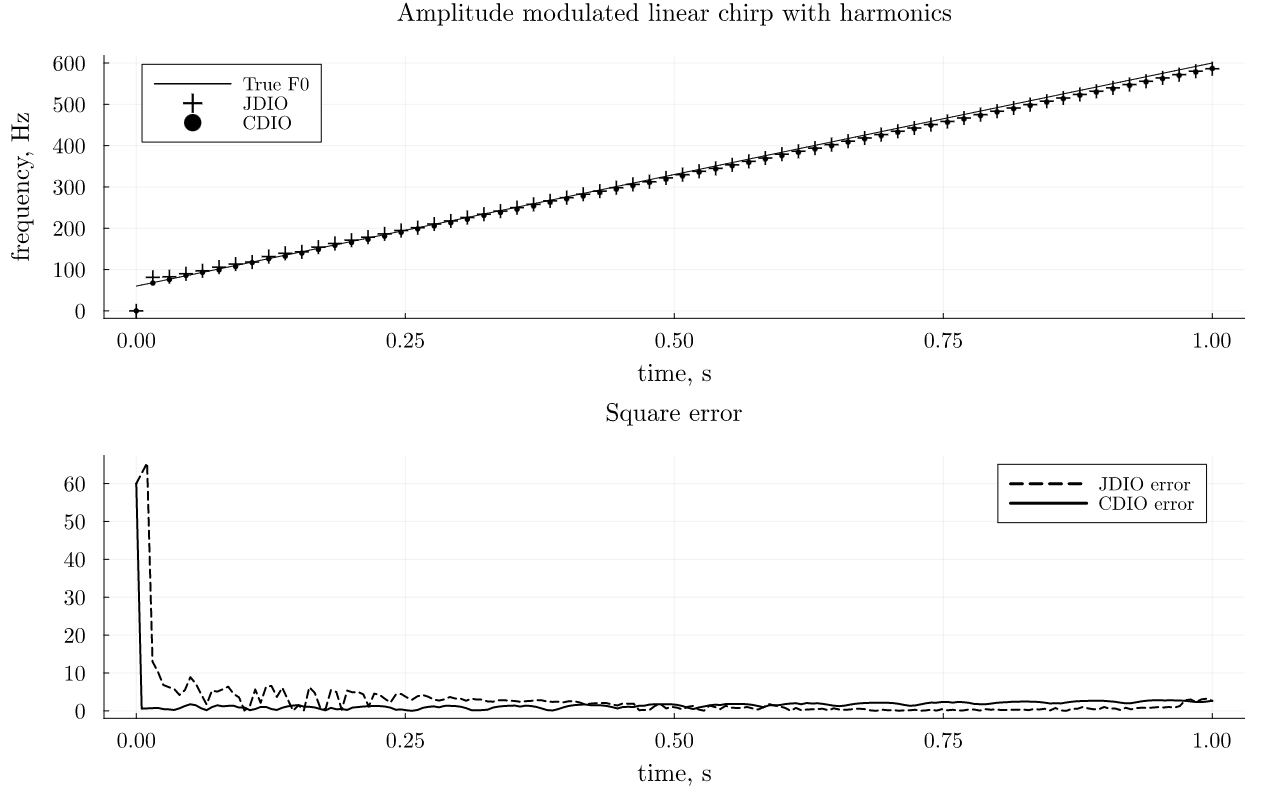
\includegraphics{graphics/amp_mod_harmonic_chirp.png}
        \caption{}
    \end{subfigure}
    \begin{subfigure}[b]{\textwidth}
        \centering
        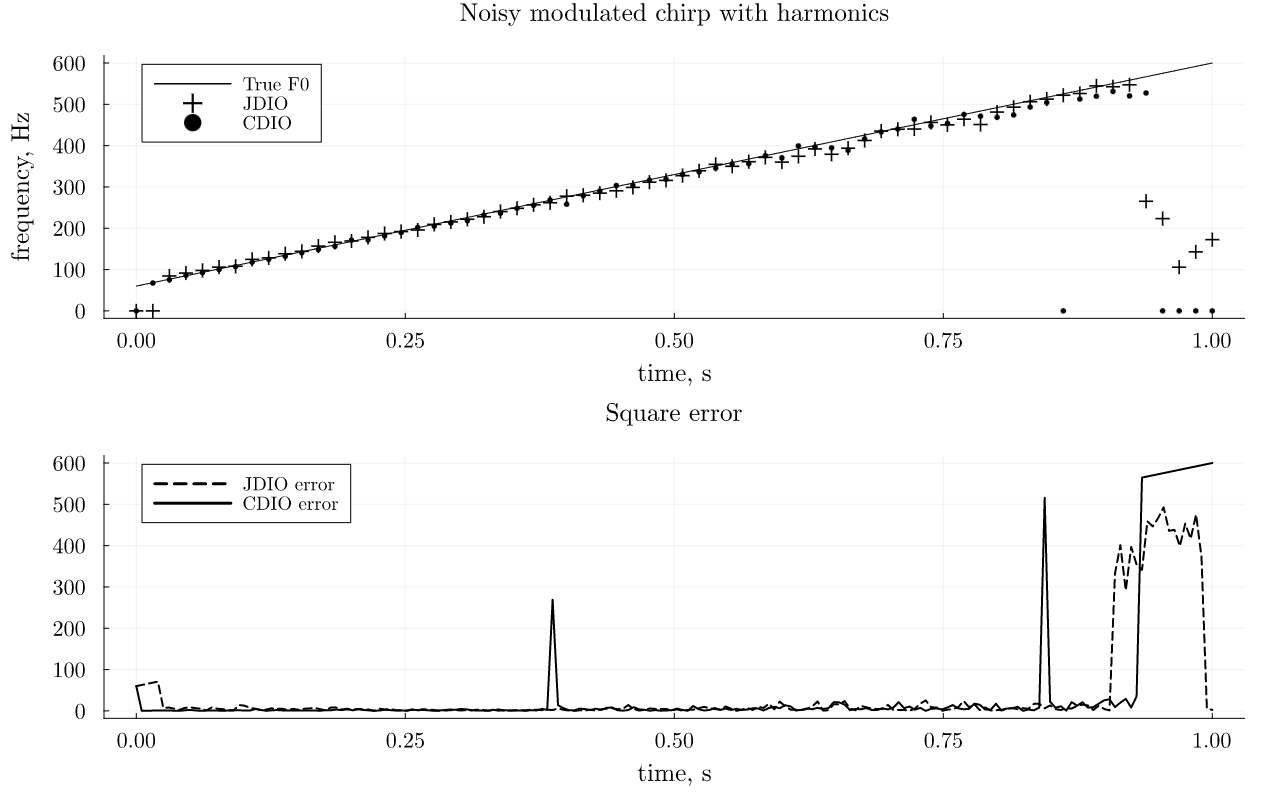
\includegraphics{graphics/noisy_harmonic_chirp.png}
        \caption{}
    \end{subfigure}
    \caption{Accuracy and errors for CDIO and JDIO when estimating the $F_0$ contour for synthesized complex harmonic signals.}
    \label{fig:f0_estimations}
\end{figure}

$F_0$ contours are easy to test because the ground truth for them is easy to obtain and compare the estimates against. The ground truth for the spectral envelopes, however, is very hard to obtain even for synthetic signals. So, to test the accuracy of JCheapTrick's implementation against CCheapTrick, an indirect approach to comparison was chosen:
\begin{enumerate}
    \item The $F_0$ contours obtained by JDIO and CDIO were used to obtain the spectrograms with JCheapTrick and CCheapTrick respectively.
    \item The aperiodicity contours were estimated for both spectrograms.
    \item The $F_0$ contours, the spectrograms, and aperiodicities were used to resynthesize the analyzed waveform using WORLD's vocoder as per Figure \ref{fig:WORLD_diagram}.
    \item Raw error was obtained by calculating the mean square deviations of the synthesized waveforms from the original sound.
    \item Spectral error was obtained by calculating the mean square deviations of the STFT spectrograms of the synthesized waveforms from the spectrogram of the original sound.
\end{enumerate}
This method also helped to demonstrate that the JDIO and JCheapTrick algorithms were compatible with the WORLD framework implementation.

Instead of the synthesized signals, real speech recordings from the LibriSpeech corpus were used for the tests. The raw errors and spectral errors calculated using the above method are provided on Figure \ref{fig:losses}.

\begin{figure}
    \begin{subfigure}[b]{0.5\textwidth}
        \centering
        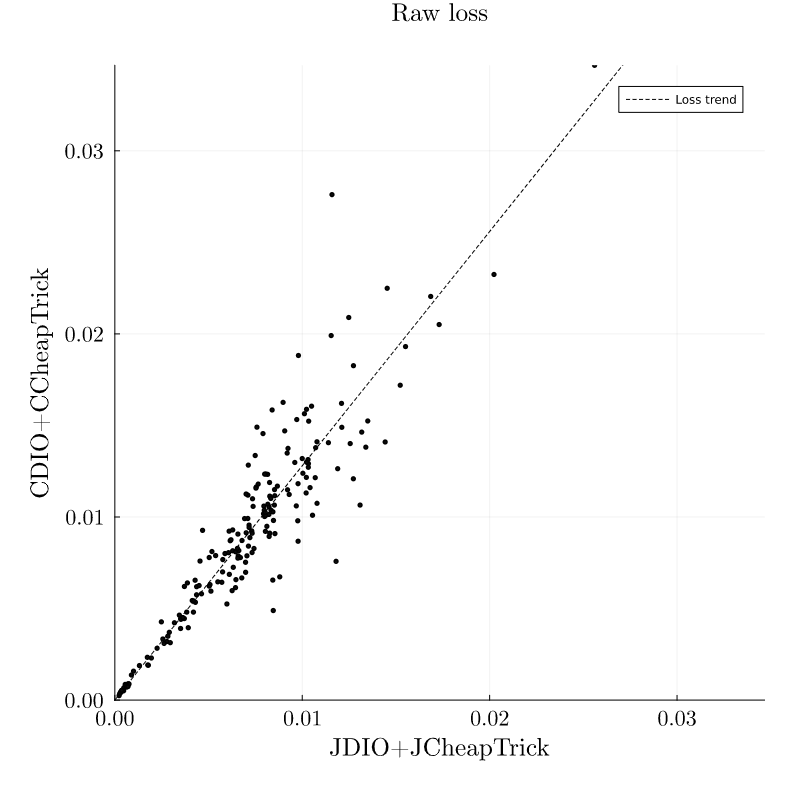
\includegraphics{graphics/raw_loss.png}
        \caption{}
    \end{subfigure}
    \begin{subfigure}[b]{0.5\textwidth}
        \centering
        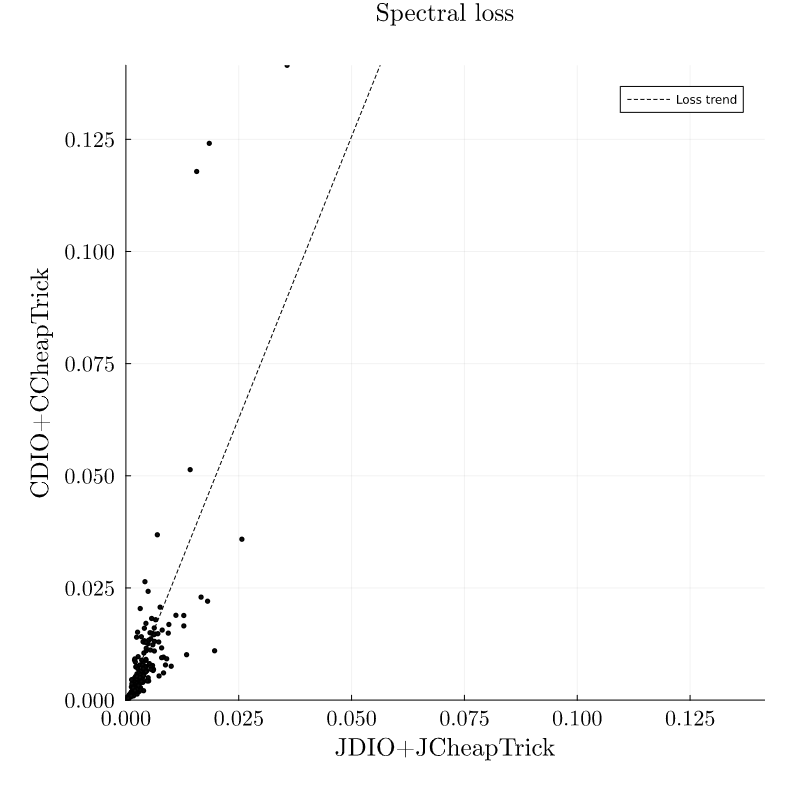
\includegraphics{graphics/spectral_loss.png}
        \caption{}
    \end{subfigure}
    \caption{Raw and spectral errors of resynthesized speech when compared to the original sound. The slopes of the mean lines are 1.27 for raw loss and 2.51 for spectral loss.}
    \label{fig:losses}
\end{figure}

The errors indicate that JDIO+JCheapTrick yielded more accurate resynthesized signal -- the raw error was $\sim1.27$ times better and the spectral characteristics of the resynthesized sound was up to $\sim2.51$ times better than for the signals resynthesized using CDIO+CCheapTrick.

\section{Conclusion}

In this paper, the implementation of the real-time DIO and CheapTrick algorithms was detailed and various accuracy and performance improvements were discussed. The new implementation was shown to have similar or better than the original implementations from the WORLD framework. The new algorithms can serve as a basis for further research and development of new real-time systems for processing speach streams.

\bibliographystyle{apacite}
\bibliography{References}

\end{document}